\documentclass[sigconf,nonacm]{acmart}

\usepackage{booktabs}
\usepackage{amsmath}
\usepackage{microtype}

\settopmatter{printacmref=false}
\renewcommand\footnotetextcopyrightpermission[1]{}
\pagestyle{plain}

\newcommand{\tool}{\textsc{Coto}}
\newcommand{\aaqdd}{AAQDD}
\newcommand{\C}{\mathbb{C}}
\newcommand{\norm}[1]{\left\lVert #1\right\rVert}

\title{Sound Memory-Bounded Quantum Simulation with Abstract Additive Decision Diagrams}

\author{Malo Leroy}
\author{Renaud Vilmart}

\begin{document}

\begin{abstract}
Classical simulation is indispensable for developing quantum programs, but explicit state
vectors require exponential memory and exact decision diagrams can lose compression on
unfavourable circuits. We introduce abstract additive quantum decision diagrams
(\aaqdd{}s), a representation that combines shared decision-diagram structure, multiple
additive branches, and rectangular complex intervals. A user-supplied per-level node budget
triggers sound joins, trading structural memory for precision while allowing simulation to
continue. Because correlation-insensitive interval propagation is easily unsound, the
implementation separates a useful nominal midpoint from a certificate: for a unitary circuit
with exact state $\psi$ and reported midpoint $m$, it encloses the result using the universal
bound $\norm{\psi-m}_2 \leq 1+\norm{m}_2$.

We implement the method in the C++23 simulator \tool{} and evaluate it against Qiskit Aer's
state-vector method and MQT DDSIM. Every one of 48 exact and approximate validation runs
contains every reference amplitude. On an eight-qubit adversarial circuit, one setting
achieves midpoint fidelity $0.651$, while another reduces stored diagram structure from
$3.00$ to $1.32$ MiB. On a deeper 30-qubit adversarial circuit, the bounded modes complete
under fixed 10-second and 4-GiB limits where dense and exact decision-diagram baselines do
not. The present certificate is deliberately conservative and useful nominal propagation is
limited to eight qubits; accordingly, the contribution is a sound memory-bounded mechanism
and reproducible reachability result, not a uniformly monotone accuracy curve.
\end{abstract}

\keywords{quantum circuit simulation, decision diagrams, abstract interpretation,
interval arithmetic, approximate computing, reproducibility}

\maketitle

\section{Introduction}

An $n$-qubit pure state has $2^n$ complex amplitudes. Dense state-vector simulators are
therefore predictable but encounter an exponential memory wall. Decision diagrams instead
share repeated substructure and can represent states such as GHZ or separable products in
space polynomial in $n$; their performance, however, depends strongly on circuit structure
and simulation order~\cite{wille2022tools,burgholzer2022paths}. Existing approximate
decision-diagram techniques commonly discard low-weight contributions while targeting an
empirical fidelity~\cite{zulehner2020approximation}. This is valuable, but it does not by
itself provide a component-wise sound enclosure of the exact state.

Our starting point is different: when an exact diagram exceeds a memory policy, continue in
an abstract domain that contains the exact computation. The idea follows abstract
interpretation~\cite{cousot1977abstract}: replace exact complex coefficients by sets of
coefficients, and replace structurally distinct subgraphs by a join. A result then carries
quantified uncertainty rather than silently becoming an unqualified approximation. The
engineering difficulty is preserving both soundness and usefulness. Additive diagrams expose
correlations between branches; naively joining edge intervals or applying gates to already
merged branches can cancel uncertainty and become unsound. Conversely, repeatedly applying
global interval matrix bounds is sound but rapidly destroys the midpoint.

This paper makes four contributions:

\begin{itemize}
  \item We define \aaqdd{}s, whose additive interval-labelled edges represent sets of
  state vectors.
  \item We give a memory policy that caps nodes at every nonterminal level and a sound general
  join for additive contexts.
  \item We separate nominal propagation from a simple, independently checkable unit-norm
  certificate, and state precisely where the implementation falls back to a coarse enclosure.
  \item We provide an open implementation, isolated baseline comparisons, raw data, figures,
  tests, and one-command build and experiment targets.
\end{itemize}

The evaluation answers three questions: whether returned rectangles contain exact reference
amplitudes (RQ1), whether budgets expose a measurable memory--precision trade-off (RQ2), and
whether bounded abstraction reaches circuits that exceed exact methods under identical
resource limits (RQ3).

\section{Background and Representation}

\subsection{Quantum states and decision diagrams}

Let $\psi\in\C^{2^n}$ be an $n$-qubit state with $\norm{\psi}_2=1$. A gate on $k$ qubits is
embedded as a unitary transformation $U$, and circuit simulation computes
$\psi_t=U_t\cdots U_1\lvert 0^n\rangle$. A quantum decision diagram recursively decomposes a
vector by qubit and shares equal sub-vectors. Weighted edges factor complex amplitudes;
canonical normalization permits extensive sharing on structured states. The same mechanism
can nevertheless approach the dense representation on unstructured states.

\tool{} uses an additive variant. At height $h>0$, a node contains finite multisets of left
and right edges $(a_i,D_i)$, where each child has height $h-1$. Its evaluation concatenates
two sums:
\begin{equation}
 \mathcal E_h(L,R)=
 \begin{pmatrix}
   \sum_{(a,D)\in L} a\,\mathcal E_{h-1}(D)\\
   \sum_{(a,D)\in R} a\,\mathcal E_{h-1}(D)
 \end{pmatrix},
 \qquad \mathcal E_0(\boxed{1})=1.
 \label{eq:evaluation}
\end{equation}
Multiple edges to shared children make sums explicit and are useful during gate rewriting.

\subsection{Rectangular complex intervals}

An abstract coefficient is a closed rectangle
$A=[r_-,r_+]+i[s_-,s_+]\subseteq\C$. Interval addition and multiplication outwardly round
their endpoints. Replacing every $a$ in Equation~\ref{eq:evaluation} by such an $A$ yields a
set-valued evaluation $\mathcal E^\sharp(D)$. We order diagrams by concretization:
$D_1\sqsubseteq D_2$ when $\mathcal E^\sharp(D_1)\subseteq
\mathcal E^\sharp(D_2)$ component-wise. A reduction is sound if $D\sqsubseteq R(D)$.

This representation differs from attaching one error scalar to a conventional diagram.
Intervals can express asymmetric real and imaginary uncertainty locally, while additive
branches retain alternatives created by rewriting. They also expose the central hazard:
independently varying occurrences of an interval loses correlations, and later algebraic
cancellation cannot be assumed.

\section{Memory-Bounded Abstract Simulation}

\subsection{Budgeted reduction}

After each gate, the simulator counts reachable nodes at every nonterminal height. Given a
budget $B\geq1$, it repeatedly selects two nodes from an over-budget level using a
minimum-imprecision heuristic and redirects their parents to a merged node. The policy ends
when each such level has at most $B$ nodes. $B$ is therefore a structural control, not a
direct byte limit: edge-vector capacity and the number of additive branches remain visible in
the measured footprint.

For non-additive contexts, one might join corresponding edge coefficients. That construction
is not sound in the general additive case because the same child can participate in several
sums. \tool{} instead evaluates a global complex enclosure for each merge operand, joins the
two enclosures, and constructs a uniform diagram whose every amplitude is contained by the
joined rectangle. This loses precision but is monotone under arbitrary incoming additive
coefficients. Parent links are rebuilt before reduction so replacement is scoped to the
owned root, and dead branches are removed without deleting shared live children.

\subsection{Nominal propagation and certification}

A uniform enclosure propagated through many gates using interval row bounds becomes enormous
and has zero midpoint. For small diagrams, \tool{} therefore propagates the reduced structure
as a \emph{nominal} interval diagram. That midpoint is useful empirically, but the structural
intervals alone are not trusted as a sound certificate after correlation-sensitive rewrites.

Instead, let $m$ be the vector of component-wise rectangle midpoints after nominal
propagation. Every supported circuit gate is unitary and the initial state is normalized, so
$\norm{\psi}_2=1$. The triangle inequality gives
\begin{equation}
  \norm{\psi-m}_2 \leq \norm{\psi}_2+\norm{m}_2=1+\norm{m}_2=:\varepsilon.
  \label{eq:certificate}
\end{equation}
For each component $j$, both
$|\operatorname{Re}(\psi_j-m_j)|\leq\varepsilon$ and
$|\operatorname{Im}(\psi_j-m_j)|\leq\varepsilon$. The machine-readable result is therefore
the outward-rounded rectangle
\begin{equation}
 [\operatorname{Re}m_j-\varepsilon,\operatorname{Re}m_j+\varepsilon]
 +i[\operatorname{Im}m_j-\varepsilon,\operatorname{Im}m_j+\varepsilon].
\end{equation}

\noindent\textbf{Proposition 1.} \emph{For a supported unitary circuit, every exact output
amplitude belongs to its reported certified rectangle.}

\noindent\emph{Proof.} Equation~\ref{eq:certificate} bounds the Euclidean norm of the error.
The magnitude of each component, and hence each of its real and imaginary parts, is no larger
than that norm. Outward rounding can only enlarge the resulting rectangle. \hfill$\square$

The certificate is universal but weak: even a good midpoint may receive a bound near two.
It is intentionally reported separately from midpoint fidelity. Nominal propagation is
limited to eight qubits, based on the measured onset of interval-branch explosion. Once a
larger diagram becomes abstract, subsequent gates use a compact uniform unitary-image
enclosure. Exhaustive certified output is capped at 16 qubits; structural measurements have
no such serialization requirement.

\section{Implementation}

\tool{} is a C++23 file-mode and interactive OpenQASM simulator. It supports common one-,
two-, and three-qubit unitary gates, parameterized rotations, global phase, and a universal
single-qubit gate. OpenQASM 3 provides the surrounding circuit syntax~\cite{cross2022openqasm}.
The directives \texttt{@reduce(B)}, \texttt{@exact}, \texttt{@memory}, and
\texttt{@intervals} control reduction and machine-readable output.

Structural memory counts each reachable node once and includes allocated edge-vector and
parent-vector capacities. It excludes allocator overhead; the comparative harness separately
records peak resident set size (RSS) using GNU \texttt{time}. The analysis layer transpiles a
supported OpenQASM 2 subset, removes final measurements, and rejects classical control rather
than changing it silently.

Correctness checks cover interval arithmetic, gate conventions, qubit ordering, shared-node
ownership, duplicate additive branches, deterministic reduction properties, enclosure, and
large-circuit memory safeguards. The release and ASan/UBSan configurations each execute 121
tests; 32 Python tests cover parsing, transpilation, isolation, resource classification, and
Aer/DDSIM integration.

\section{Evaluation}

\subsection{Protocol}

Experiments ran on Linux x86-64 with 16 logical CPUs. The checked metadata records Python
3.13.11, Qiskit 2.5.2, Qiskit Aer 0.17.2, and MQT DDSIM 2.5.0. Each comparative configuration
runs in a fresh process with a 10-second wall-time limit and 4-GiB address-space limit, repeated
three times. Aer uses its state-vector simulator~\cite{qiskitaer}; MQT uses its decision-
diagram QASM simulator~\cite{mqtddsim}; both execute one measured shot. \tool{} runs exact and
with $B\in\{1,4,16\}$. Successful plots use medians and never turn failures into numeric
points.

The 22 circuits comprise scalable separable and GHZ families (10--60 qubits), four-layer
deterministic entangling circuits (6--12 qubits), two deep adversarial circuits (20 and 30
qubits, 20 layers), and four small QASMBench kernels~\cite{li2021qasmbench}. The deep circuits
apply seeded $R_x/R_y/R_z$ rotations to every qubit and alternating nearest-neighbour CNOTs.
They are explicitly contrived to erode exact decision-diagram sharing.

For RQ1 and RQ2, Aer computes exact vectors for separable, GHZ, layered 6/8-qubit, and four
QASMBench instances. \tool{} runs exact and with $B\in\{1,2,4,8,16\}$. We reverse state
indices to account for Coto's most-significant-bit convention, then record component
containment, normalized midpoint fidelity
$|\langle\psi/\norm\psi,m/\norm m\rangle|^2$, midpoint error, rectangle diameters, and the
certificate of Equation~\ref{eq:certificate}.

\subsection{Resource scaling and reachability}

\begin{figure}[t]
  \centering
  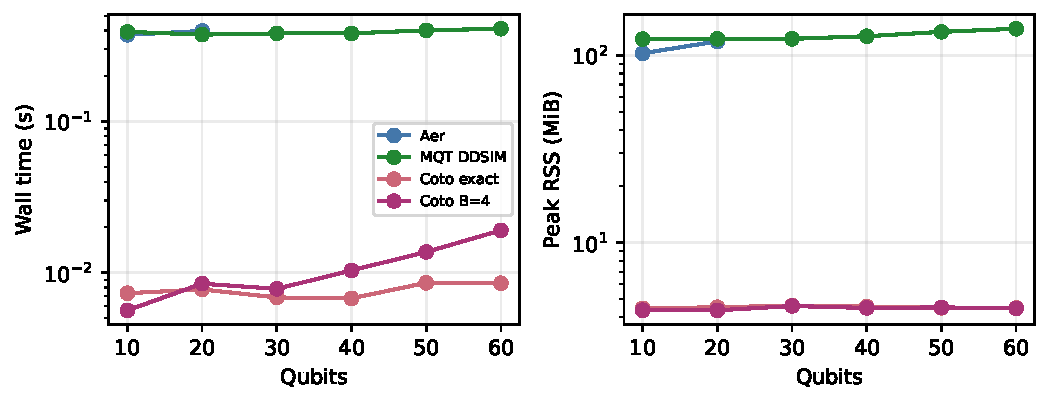
\includegraphics[width=\columnwidth]{../analysis/results/figures/scaling.pdf}
  \Description{Two log-scale line charts show wall time and peak RSS versus qubits for Aer,
  MQT DDSIM, exact Coto, and budget-4 Coto on separable circuits.}
  \caption{Median whole-process time and peak RSS on separable states. Missing Aer points hit
  the 4-GiB address-space limit. DD methods compress this favourable family.}
  \label{fig:scaling}
\end{figure}

Figure~\ref{fig:scaling} first provides a sanity check. At 60 qubits, Aer exceeds the memory
limit, MQT DDSIM completes in roughly $0.4$ s with about 139 MiB RSS, and exact \tool{}
completes in about $0.009$ s with 12.3 KiB of stored structure. GHZ shows the same qualitative
result. These favourable families demonstrate compression but not a unique advantage over
existing DD simulation.

The layered cases expose the distinction. Exact \tool{} times out at 10 and 12 qubits, while
all bounded modes complete in milliseconds using only a few KiB after the large-circuit
safeguard. The deep 20-qubit case is still tractable for Aer but times out in MQT DDSIM. At 30
qubits, Aer crosses the memory limit and MQT DDSIM and exact \tool{} time out; bounded
\tool{} completes. Table~\ref{tab:deep} reports the final medians and statuses.

\begin{table}[t]
  \caption{Deep adversarial circuits under 10 s and 4 GiB. Times are medians of successful
  runs; failures occurred in all three repetitions.}
  \label{tab:deep}
  \centering
  \begin{tabular}{llrr}
    \toprule
    Qubits & Engine/configuration & Time (s) & Structure \\
    \midrule
    20 & Aer state vector & 0.652 & --- \\
    20 & MQT DDSIM & timeout & --- \\
    20 & \tool{} exact & timeout & --- \\
    20 & \tool{} $B=4$ & 0.0127 & 4.42 KiB \\
    30 & Aer state vector & memory & --- \\
    30 & MQT DDSIM & timeout & --- \\
    30 & \tool{} exact & timeout & --- \\
    30 & \tool{} $B=4$ & 0.0270 & 6.70 KiB \\
    \bottomrule
  \end{tabular}
\end{table}

Thus RQ3 is positive for the deliberately adverse 30-qubit instance: within the stated
limits, bounded abstraction returns a sound structural enclosure where both selected
alternatives fail. This is a reachability statement, not a claim that it returns a precise
state estimate at that scale.

\subsection{Soundness and memory--precision behaviour}

All 48 validation rows have containment rate 1.0: every exact Aer amplitude lies in the
reported rectangle (RQ1). Exact rows have fidelity one and zero certificate radius up to
floating-point noise. Approximate rows exercise all five budgets and repeated reductions.

\begin{figure*}[t]
  \centering
  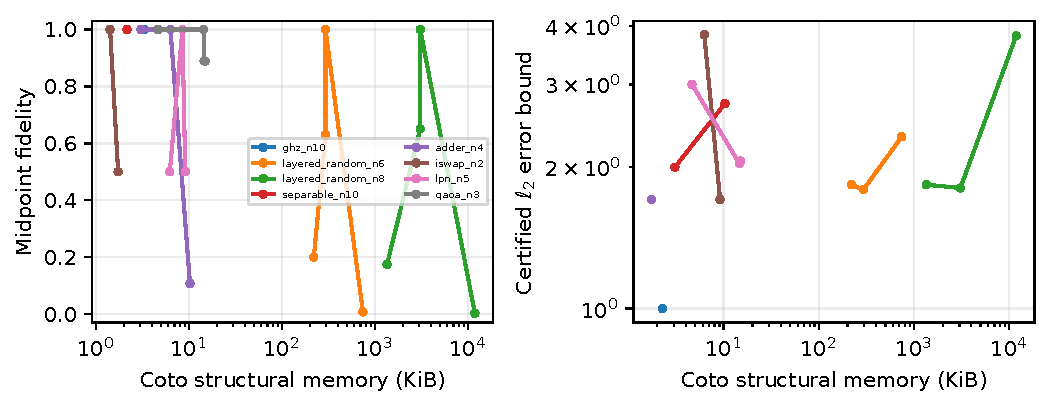
\includegraphics[width=0.82\textwidth]{../analysis/results/figures/tradeoff.pdf}
  \Description{Two scatter-line charts show midpoint fidelity and certified L2 error bound
  versus Coto structural memory for eight validation circuits.}
  \caption{Empirical midpoint fidelity (left) and the independently certified $\ell_2$ error
  bound (right) versus stored \tool{} structure. Lines connect configurations sorted by
  memory, not by budget; nonmonotonicity is genuine.}
  \label{fig:tradeoff}
\end{figure*}

Figure~\ref{fig:tradeoff} answers RQ2 with an important qualification. On the eight-qubit
layered circuit, $B=4$ gives fidelity 0.651 with certified bound 1.807. $B=16$ stores 1.32 MiB
instead of the exact diagram's 3.00 MiB, but its fidelity is only 0.174. On the six-qubit
layered circuit, $B=16$ reaches fidelity 0.628. Several small QASMBench midpoints remain near
unit fidelity.

The relationship is not monotone. A smaller node cap can cause a wider merged node to create
more additive branches during later gates; budget 1 on the eight-qubit layered case is both
larger and slower than several looser settings. Selection is heuristic, so additional nodes
also need not improve the final midpoint. The data therefore demonstrate a tunable mechanism
with useful operating points, but not an ordered Pareto family. The certified bound remains
sound at every point and is kept visually separate from empirical fidelity.

\section{Related Work}

QMDD-style representations compress quantum vectors and matrices by recursive decomposition
and weighted sharing; a broad account and the tool ecosystem are given by Wille et
al.~\cite{wille2022tools}. MQT DDSIM is the closest experimental baseline. Simulation-path
research shows that contraction order alone can change DD cost by orders of magnitude
\cite{burgholzer2022paths}; our fixed sequential path leaves this optimization complementary.

Zulehner et al.~\cite{zulehner2020approximation} reduce quantum-state DDs using fidelity-
oriented schemes and report large empirical savings. \aaqdd{}s instead make uncertainty part
of the representation and prioritize set containment. The present midpoint can be compared by
the same fidelity metric, but Equation~\ref{eq:certificate} is independent of that comparison.
This resembles the sound-overapproximation discipline of abstract interpretation
\cite{cousot1977abstract}, applied to complex amplitudes and graph reduction rather than
program fixpoints.

Dense state-vector simulation remains a strong baseline because its cost is regular and its
semantics straightforward. Aer also offers several non-dense methods, but we deliberately
select its state-vector mode to expose the memory wall and pair it with DDSIM to avoid treating
all structural simulation as new. QASMBench supplies externally defined kernels; the
adversarial circuits serve a different, clearly labelled purpose by isolating failure modes.

\section{Threats to Validity and Limitations}

The certificate is mathematically sound but too loose to establish practical accuracy; for an
abstract result it is at least one and often near two or more. Deriving a tighter compositional
error bound is the main research problem left open. Above eight qubits the safeguarded midpoint
is zero, so large reachability results say only that a sound enclosure was computed. Certified
amplitude serialization is limited to 16 qubits.

The benchmark uses one measured shot and includes unequal process startup: Aer and DDSIM load
Python packages, while \tool{} is native. The CSV provides Python-engine simulation time, but
whole-process comparisons remain imperfect. The 10-second cutoff is intentionally operational,
not an asymptotic result. The deep circuits are seeded and reproducible but contrived; real
workload distributions may behave differently. Aer has methods beyond state vectors, and MQT
offers path choices not evaluated here.

The supported language is unitary-only. Mid-circuit measurement, noise, and classical control
are outside scope. Finally, 100\% containment on 48 rows plus deterministic property tests is
strong validation, not a mechanized end-to-end proof. The repository's author-review report
lists these limitations and open engineering bugs explicitly.

\section{Reproducibility}

The repository contains source, pinned QASMBench data, raw per-process CSV rows, metadata,
plot generation, and the manuscript. The recorded implementation commit is \texttt{2bec253};
its full hash is in the metadata. From \texttt{paper/},
\texttt{nix-shell --run 'make pdf'} builds this document with ACM's \texttt{acmart} class.
\texttt{make verify} builds and tests the simulator; \texttt{make experiments} reruns the
bounded collectors and figures. Metadata records versions, limits, repetitions, platform,
and the implementation commit; failed rows remain in the raw data.

\section{Conclusion}

\aaqdd{}s turn a fixed structural budget into a sound continuation strategy for quantum
simulation. The implementation never equates a high-fidelity midpoint with a guarantee:
nominal quality is measured empirically, while a separate unit-norm argument certifies every
reported amplitude rectangle. The experiments find useful small-circuit midpoints, expose
nonmonotone heuristic behaviour, and show a 30-qubit adverse circuit reachable within fixed
limits after both dense and exact-DD alternatives fail. The next step is not a larger claim,
but a tighter compositional certificate and a merge policy that makes precision and memory
more predictably monotone.

\bibliographystyle{ACM-Reference-Format}
\bibliography{references}

\end{document}
